\documentclass[../../main]{subfiles}

\begin{document}

\paragraph{Abstract}

The inductance of the two motors controlling the pan-tilt system is determined.

\paragraph{Introduction}

The electrical inductance of the motors are determined in this journal. Every constant concerning the motor of the top frame is denoted $A_t$ while the constants for the buttom frame is denoted $A_b$.

\paragraph{Materials and Methods}

To determine the electrical inductance of the two motors, the time constant method is used.\\
Firstly the motor, illustrated as a coil, is linked in series with a resistor and a PWM controlled MOSFET. This can be seen on figure \ref{fig:inductance_circuit}. By rapidly switching the MOSFET on and off the coil inside the motor will be charged and discarged along with current flowing through the resistor. This will cause a wave pattern to show the voltage across the coil. Using an oscilloscope, the time from the wave starting to the top of the wave is given as:
$$\tau = \frac{L}{R}$$

\begin{figure}[h]
  \begin{center}
    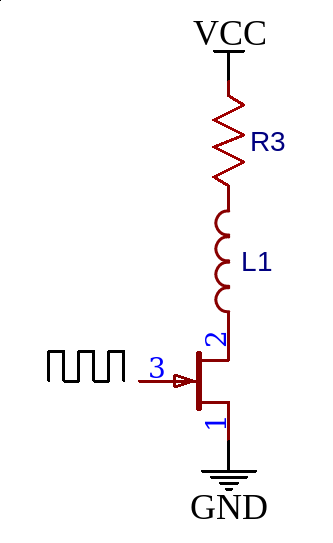
\includegraphics[width=0.3\textwidth]{\main/journaler/journal_L/circuitDiagramL.png}
  \end{center}
    \caption{Circuit diagram for the experiemnt}
    \label{fig:inductance_circuit}
\end{figure}

By applying this method the time constant is determined to be $\tau = 17.5 \cdot 10^{-6}s$. Thus the inductance with a resistor of size $22\Omega$ can be determined:\\
$$L = 17.5 \cdot 10^{-6}s \cdot 22 \Omega = 3.85 \cdot 10^{-4}H$$
The time constant was measured to be approximitly equal for both motors, which results in the following being true::\\
$$L_b=L_t=3.85 \cdot 10^{-4}H$$

\paragraph{Results}

The result of this experiment is:
$$L_b = 3.85 \cdot 10^{-4}H$$
$$L_t = 3.85 \cdot 10^{-4}H$$

\paragraph{Conclusion}

The electrical inductance of the motor controlling the top frame is $L_t= 3.85 \cdot 10^{-4}H$ and the resistance of the motor controlling the buttom frame is $L_b= 3.85 \cdot 10^{-4}H$.










\end{document}
